\chapter{Применение} \label{chapt3}
\section{Распознавание символов}
Наиболее естественным применением разработанного подхода является, очевидно, распознавание символов (букв, логотипов и т.п.).

Рассмотрим метод на примере анализа буквы <<a>>

...

Отдельно стоит упомянуть задачу поиска партизана в лесу

...
\section{Оценка устойчивости битумных эмульсий}
\subsection{Введение}
В настоящее время трудно назвать область строительства, где бы не применялись эмульсии. Они используются в дорожном и в гражданском строительстве в качестве связующих с различными наполнителями, а также в качестве гидроизоляционных и лакокрасочных материалов. При любых технологиях использования эмульсий мы сталкиваются с одними и теми же проблемами, касающимися подбора состава, приготовления, определения физико-механических характеристик, стабильности, контроля распада эмульсий и получения продукции с необходимыми свойствами [1]. Далее мы будем рассматривать только прямые битумные и битумно-латексные эмульсии, которые являются наиболее крупнотоннажным продуктом: мировое использование составляет миллионы тонн в год

Традиционные методы оценки свойств битумных эмульсий включают: определение содержания вяжущего с эмульгатором, определение устойчивости эмульсии при перемешивании, определение остатка на сите, определение условной вязкости, определение устойчивости при хранении, определение адгезии эмульсий с поверхностью наполнителей, определение устойчивости при транспортировки и т.п. [2].  Наряду с традиционными методами изучения  качества эмульсии, во многих приложениях желательно знать более тонкие характеристики, например: функцию распределения по размерам. Эта характеристика является одним из важнейших параметров и позволяет предсказывать большинство свойств эмульсии. Обычноразмер частиц оценивают с помощью определения остатка на сите с заданным размером ячейки, но такой метод позволяет оценивать только верхний предел размеров частиц эмульсии. Полная картина распределения частиц по размеру может быть измерена с использованием таких технических приёмов как рассеяние света, микроскопия с анализом изображений, или же с помощью техники электроозонирования («техники Культера» - Coulter). Точный анализ размеров частиц битумной эмульсии может решить многие проблемы, которые в настоящее время являются актуальными в сфере производства битумных эмульсий:
\begin{enumerate}
\item Влияние эмульгатора и его концентрации на размер битумных частиц эмульсии.
\item Влияние модифицирующих битум добавок на качество получаемой эмульсии.
\item Корректировка технологической схемы производства эмульсии.
\item Влияние размера битумных частиц на основные физические свойства эмульсии.
\end{enumerate}

Оптическая микроскопия, как способ распределения частиц по размерам, является наиболее удобным и точным.Например, если в способе «рассеяние света» могут возникнуть проблемы с отражением света от черных поверхностей, какими являются частицы битума, то в способе микроскопии, при высоком контрасте черного цвета, напротив, можно отличить частицы от среды, в которой они находятся.

\begin{figure}[h]
	\centering
	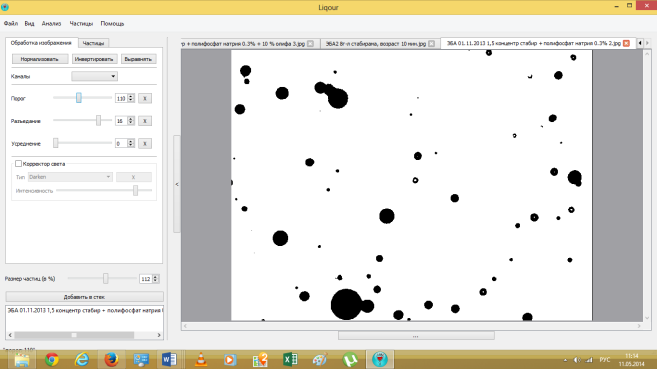
\includegraphics{images/em_00}
\end{figure}

Очевидно изображения такого вида являются одним из примеров растровых контурных изображений, с несколькими контурами. В отличие от задачи распознавания символов, здесь нет необходимости анализировать скелет изображения. Куда более важную роль играет внешний контур. Разбивая контур на дуги мы можем классифицировать частицы по уровню распада:
\begin{enumerate}
\item одиночные
\item слипшиеся
\item распавшиеся
\end{enumerate}
Большое количество распавшихся частиц является свидетельством того что смесь является неустойчивой, а следовательно некачественной.

\subsection{Анализ эмульсий}
В результате сотрудничества с кафедрой <<Автомобильных дорог>> НИ ИрГТУ была разработана программа для первичной оценки качества битумных эмульсий

\begin{figure}[h]
	\centering
	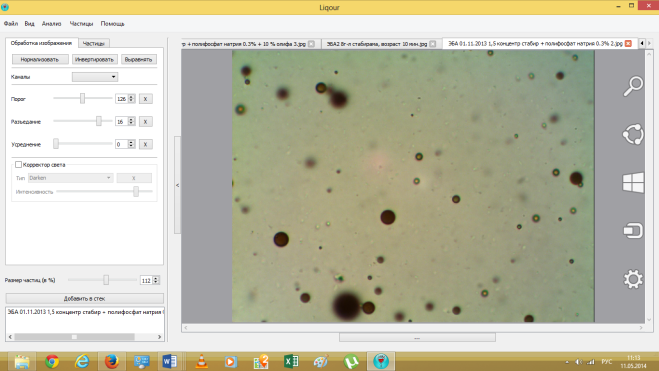
\includegraphics{images/em_03}
	\caption{Скриншоты программы «анализ изображений»}
	\label{em_img_program}
\end{figure}

\begin{figure}[h]
	\centering
	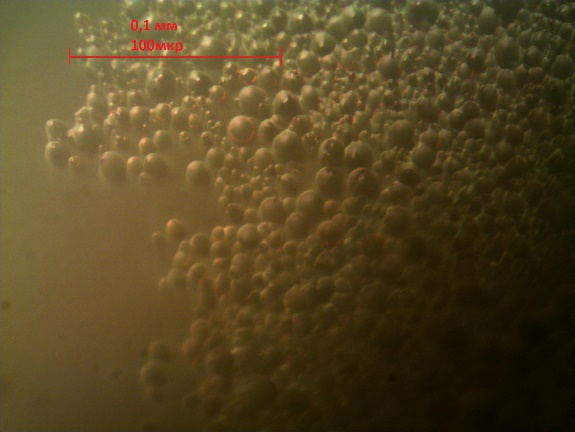
\includegraphics{images/em_01}
	\caption{Концентрированная битумная анионная эмульсия в отраженном свете}
	\label{em_img_bad}
\end{figure}

На снимке программы (рис. \ref{em_img_program}), видно, что в проходящем свете частицы легко отличить друг от друга, но для получения такого изображения необходимо создать некоторое пространство между ними, в противном случае изображение получатся как на рис. \ref{em_img_bad}. Поэтому перед микроскопическими исследованиями образцы эмульсии распределяют небольшим количеством (концентрация от 1:100 – 1:50) в специальном стабилизирующем растворе. Необходимость данной процедуры объясняется тем что, частицы битума могут слипаться под стеклышком и отсутствие сцепления между ними осуществляется за счет pH среды, в которой они находятся. Для анионных эмульсий это pH-щелочной, для катионных pH-кислотный.

Гибкость настроек программы позволяет редактировать изображение вручную, убирая «мнимые частицы», затемненные области и другие недочеты фотосъемки. После чего происходит автоматический подсчет частиц и построение графика функции распределения по размерам, рис. 5. 

Для данной программы не требуется специализированного оборудования. Достаточно оптического микроскопа с возможностью подключения цифровой камеры и компьютер с ОС (Windows, Linux, OS).

\subsection{Оценка качества анализа}

\begin{figure}[ht]
	\centering
	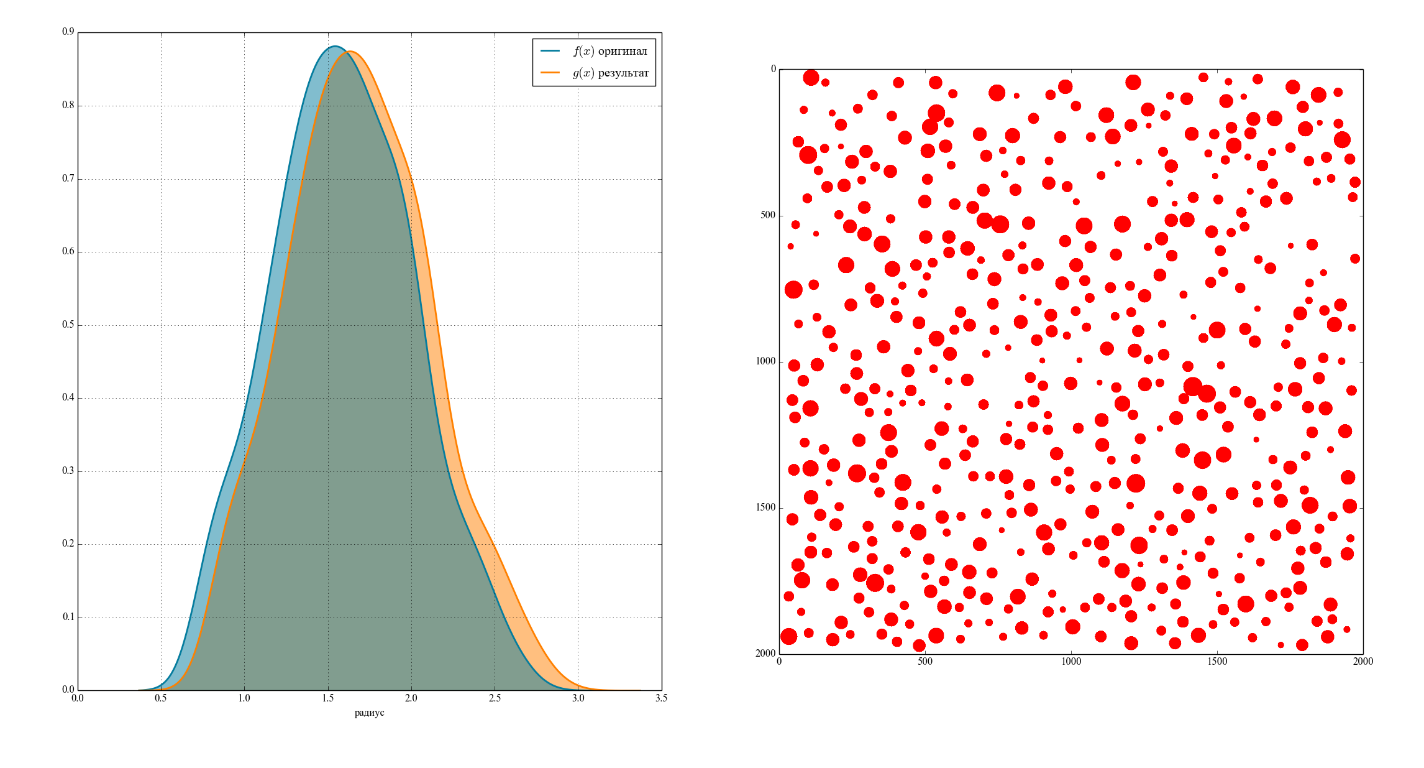
\includegraphics{images/em_07}
	\caption{Результат работы программы на искусствено сгенерированных данных}
	\label{em_artifical}
\end{figure}

На рисунке (рис. \ref{em_artifical}) приведены два графика: тот что сильнее смещен влево – соответствует исходным авто-сгенерированным данным, смещенный вправо соответствует распознанным данным. Формы графиков практически идентичны. Смещение, как правило, вызвано ошибками округления при распознавании объектов.

\begin{table}[ht]
  \centering
  \caption{Анализ распределения частиц на рис. \ref{em_artifical}}
  \renewcommand{\arraystretch}{1.5}% Spread rows out...
  \begin{tabular}{*5{>{\centering\bfseries}m{1in}}>{\centering\arraybackslash}m{0.6in}}
    \toprule
	График & \textbf{мин. размер частиц, мкм.} & \textbf{макс. размер частиц, мкм.} & \textbf{Среднее значение, мкм.} & \textbf{Ср.кв. отклонение, мкм.} & \textbf{Всего частиц} \\
	\midrule
	\midrule	
	Исходный & 0.87 & 2.87 & 1.69 & 0.42 & 500 \\
	Распознанный & 0.87 & 2.69 & 1.59 & 0.41 & 493 \\
	\bottomrule
  \end{tabular}
\end{table}

\begin{figure}[ht]
	\centering
	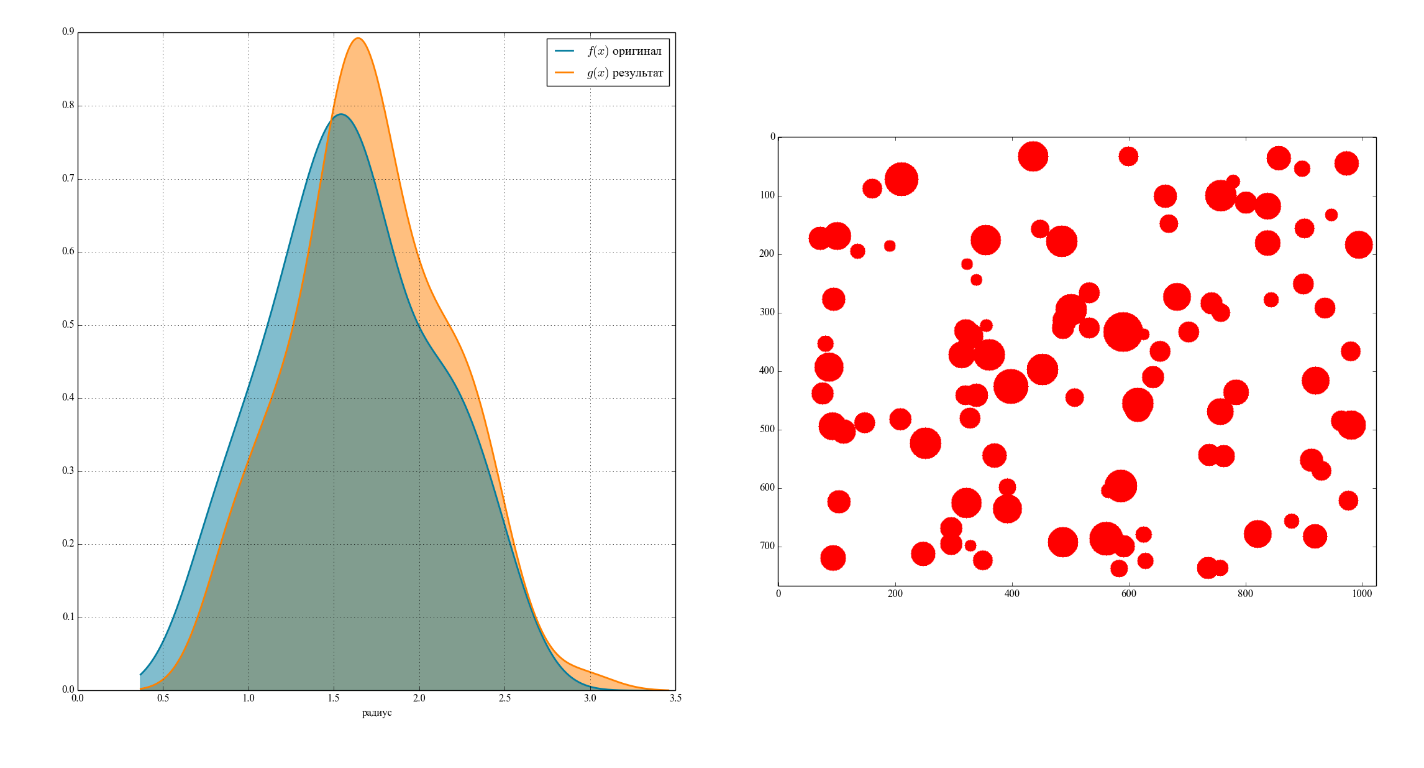
\includegraphics{images/em_04}
	\caption{Проверка работы программы при наличии слипшихся частиц}
	\label{em_merged}
\end{figure}


Вторым фактором (первый – ошибки округления) отрицательно влияющим на качество распознавания является наличие слипшихся частиц. На рис.\ref{em_merged} приведены два графика исходного (тот что более сплющен) и распознанного распределения частиц (тот что повыше). Сильное различие между графиками обусловлено тем что, при распознавании слипшиеся объекты не учитываются. 


\begin{table}[ht]
  \centering
  \caption{Распределение частиц на рис. \ref{em_merged}}
  \renewcommand{\arraystretch}{1.5}% Spread rows out...
  \begin{tabular}{*5{>{\centering\bfseries}m{1in}}>{\centering\arraybackslash}m{0.6in}}
    \toprule
	График & \textbf{мин. размер частиц, мкм.} & \textbf{макс. размер частиц, мкм.} & \textbf{Среднее значение, мкм.} & \textbf{Ср.кв. отклонение, мкм.} & \textbf{Всего частиц} \\
	\midrule
	\midrule
	Исходный & 0.87 & 2.98 & 1.71 & 0.44 & 100 \\
	Распознанный & 0.87 & 2.52 & 1.6 & 0.46 & 57 \\
	\bottomrule
  \end{tabular}
  \label{em_tbl_merged}
\end{table}

Из таблицы \ref{em_tbl_merged} видно, что, не смотря на то, что почти половина частиц не была распознана, характеристики распределения были определены достаточно точно к исходным, и погрешность составила около 4-5\%.

Получение высококачественной, долговечной битумной эмульсии зависит в основном от вязкости битума поступающего в диспергатор вместе с раствором ПАВ, а так же от скорости вращения и вида диспергирующих элементов. После выхода готовой эмульсии из диспергатора необходимо оценить её качество. 

Внешние признаки распада эмульсии видны невооруженным глазом, но если речь идет о количественном  сравнении двух визуально схожих эмульсий, то в таком случае применение программы для анализа размера частиц будет весьма кстати. 

\subsection{Определение среднего размера и дисперсии частиц битумной эмульсии на модифицированном битуме}

Стабильность эмульсии в большой степени определяется размером частиц, который в свою очередь зависит от вязкости исходного битума. Во многих практических ситуациях необходимо получать мелкие (1-5 мкм) частицы эмульсии, это даёт очень хорошую стабильность при хранении и хорошее обволакивание заполнителей. Для получения таких эмульсий необходимо специализированное дорогостоящее оборудование. 

\begin{figure}[h]
	\centering
	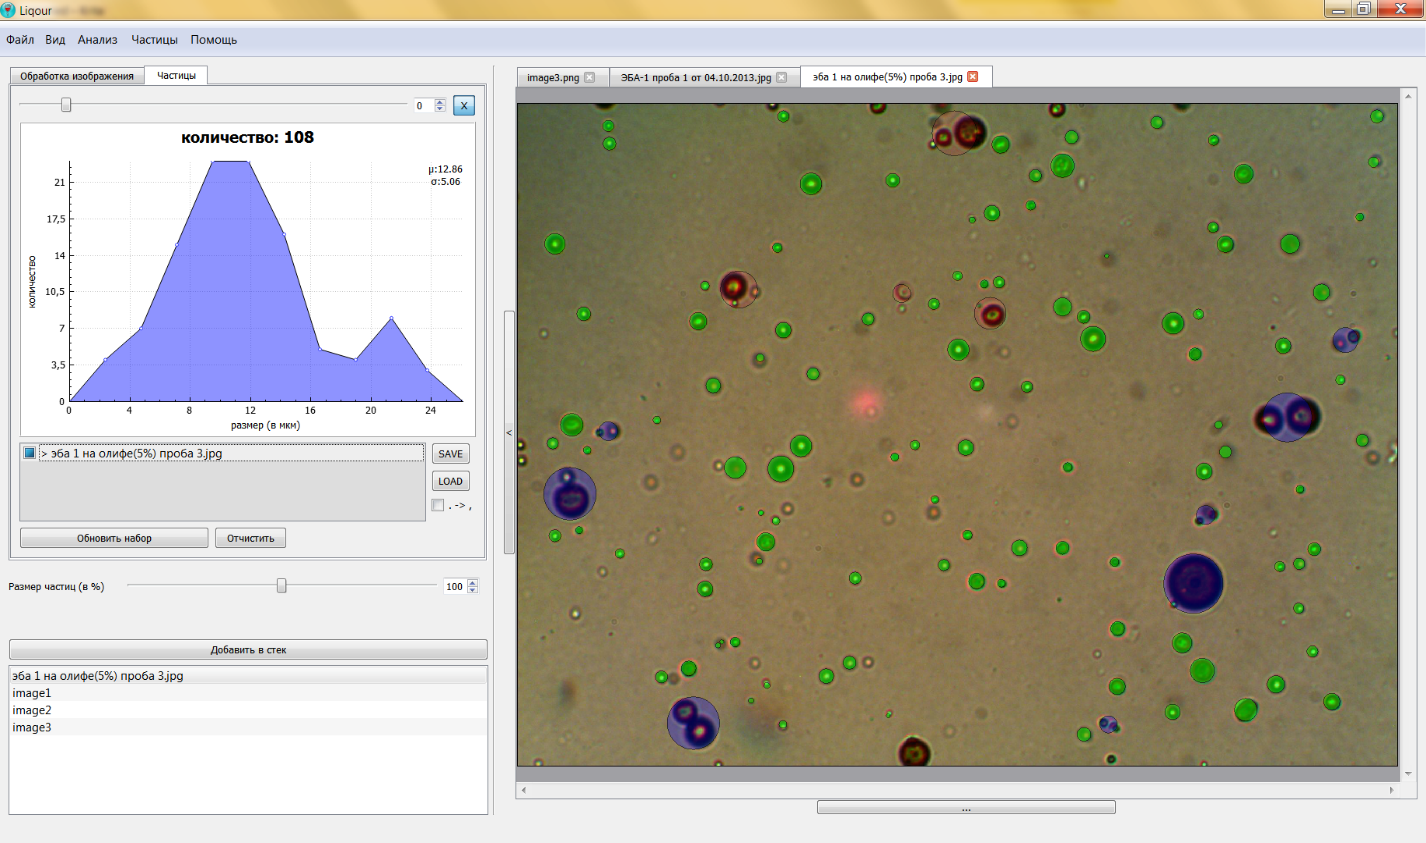
\includegraphics[scale=0.75]{images/em_05}
	\caption{ЭБА-1 на битуме разжиженном олифой (5\%)}
	\label{em_img_01}
\end{figure}

\begin{table}[h]
  \centering
  \caption{Распределение частиц на рис.\ref{em_img_01}}
  \renewcommand{\arraystretch}{1.5}% Spread rows out...Рис.9 Эмульсия, полученная в заводских условиях на вязком битуме.
  \begin{tabular}{*2{>{\centering\bfseries}m{1in}}>{\centering\arraybackslash}m{0.6in}}
    \toprule
	\textbf{Среднее значение, мкм.} & \textbf{Ср.кв. отклонение, мкм.} & \textbf{Всего частиц} \\
	\midrule
		\midrule
	12.86 & 5.06 & 108 \\
	\bottomrule
  \end{tabular}
\end{table}

Стандартные диспергаторы на которых дорожники производят битумные эмульсии позволяют получать средний размер частиц примерно 10 -20 мкм. Одним из возможных способов уменьшения размеров частиц эмульсии может являться понижение вязкости битума.
%
%\begin{figure}[h]
%	\centering
%	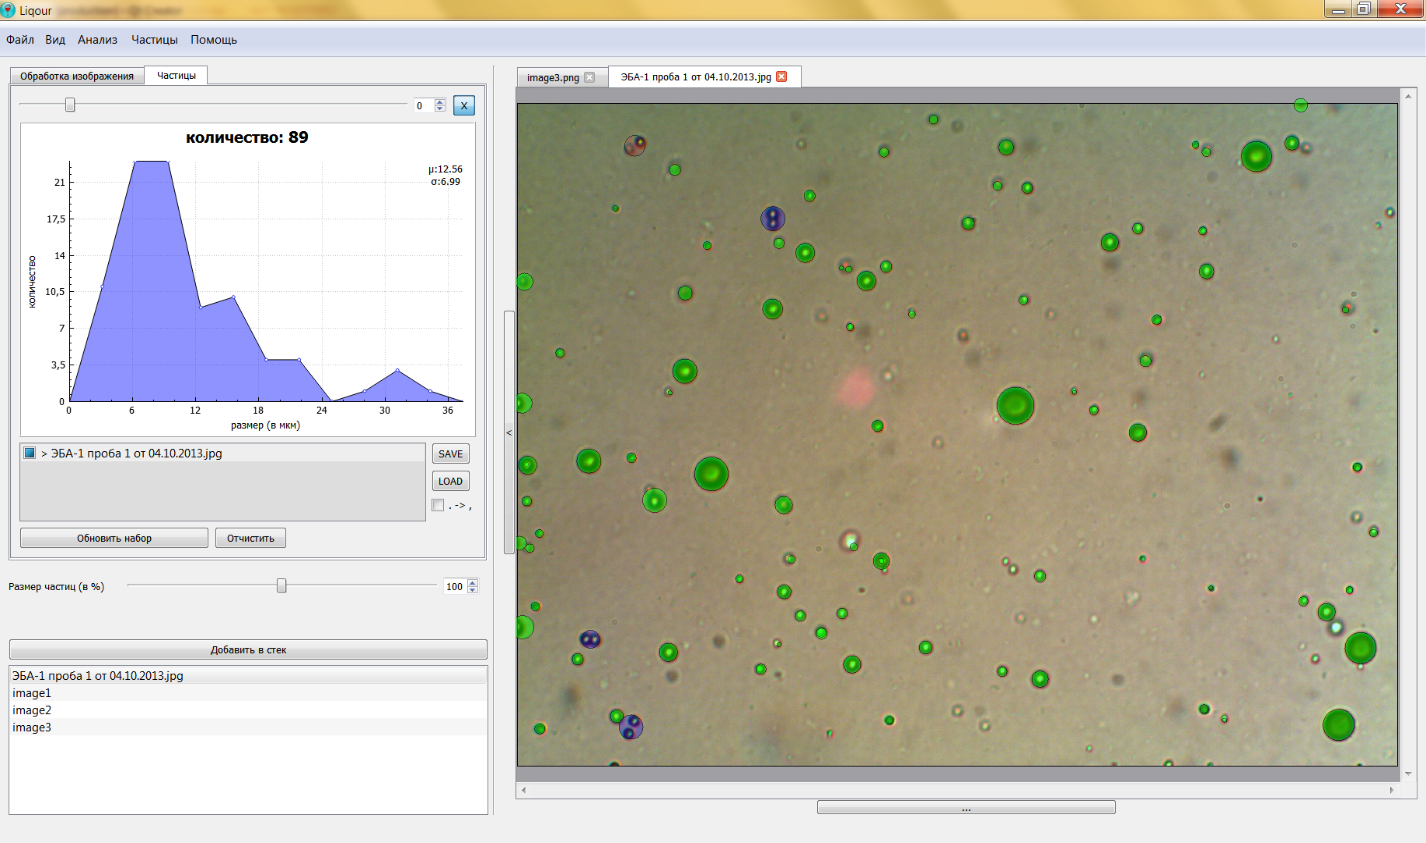
\includegraphics[scale=0.75]{images/em_06}
%	\caption{Эмульсия, полученная в заводских условиях на вязком битуме}
%	\label{em_img_02}
%\end{figure}
%
%\begin{table}[h]
%  \centering
%  \caption{Распределение частиц на рис.\ref{em_img_02}}
%  \renewcommand{\arraystretch}{1.5}% Spread rows out...Рис.9 Эмульсия, полученная в заводских условиях на вязком битуме.
%  \begin{tabular}{*2{>{\centering\bfseries}m{1in}}>{\centering\arraybackslash}m{0.6in}}
%    \toprule
%	\textbf{Среднее значение, мкм.} & \textbf{Ср.кв. отклонение, мкм.} & \textbf{Всего частиц} \\
%	\midrule
%	12.56 & 6.99 & 89 \\
%	\bottomrule
%  \end{tabular}
%\end{table}

\subsection{Результаты}
Разработанный программный комплекс, показал что изложенные выше алгоритмы отлично справляются с задачей классификации объектов по контору
...

\section{Автоматизация составления ПОДД}
%
%\section{Таблица обыкновенная} \label{sect3_1}
%
%Так размещается таблица:
%
%\begin{table} [htbp]
%  \centering
%  \parbox{15cm}{\caption{Название таблицы}\label{Ts0Sib}}
%%  \begin{center}
%  \begin{tabular}{| p{3cm} || p{3cm} | p{3cm} | p{4cm}l |}
%  \hline
%  \hline
%  Месяц   & \centering $T_{min}$, К & \centering $T_{max}$, К &\centering  $(T_{max} - T_{min})$, К & \\
%  \hline
%  Декабрь &\centering  253.575   &\centering  257.778    &\centering      4.203  &   \\
%  Январь  &\centering  262.431   &\centering  263.214    &\centering      0.783  &   \\
%  Февраль &\centering  261.184   &\centering  260.381    &\centering     $-$0.803  &   \\
%  \hline
%  \hline
%  \end{tabular}
%%  \end{center}
%\end{table}
%
%%\newpage
%%============================================================================================================================
%
%\section{Параграф - два} \label{sect3_2}
%
%Некоторый текст.
%
%%\newpage
%%============================================================================================================================
%
%\section{Параграф с подпараграфами} \label{sect3_3}
%
%\subsection{Подпараграф - один} \label{subsect3_3_1}
%
%Некоторый текст.
%
%\subsection{Подпараграф - два} \label{subsect3_3_2}
%
%Некоторый текст.
%
%\clearpage